\documentclass{beamer}
\usepackage[T2A]{fontenc}
\usepackage[utf8]{inputenc}
\usepackage[russian]{babel}
\usepackage{color}
\usepackage{hyperref}
\usepackage{listings}
\usepackage{color}
\usepackage{graphicx}
\usetheme{default}

\definecolor{javared}{rgb}{0.6,0,0}
\definecolor{javagreen}{rgb}{0.25,0.5,0.35}
\definecolor{javapurple}{rgb}{0.5,0,0.35}
\definecolor{javadocblue}{rgb}{0.25,0.35,0.75}
 
\lstset{language=Java,
    basicstyle=\ttfamily,
    keywordstyle=\color{javapurple}\bfseries,
    stringstyle=\color{javared},
    commentstyle=\color{javagreen},
    morecomment=[s][\color{javadocblue}]{/**}{*/},
    tabsize=4,
    showspaces=false,
showstringspaces=false}

\setbeamertemplate{footline}[frame number]

\title{BeanDiffer2}
\subtitle{Hamcrest Matcher}
\author{\textbf{А.~С.~Семёнов} \\ \href{mailto:semkagtn@yandex-team.ru}{semkagtn@yandex-team.ru}}
\institute{\textbf{\textcolor{red}{Я}ндекс}}
\date{\today}

\subject{QA-engenier programing tools}

\AtBeginSubsection[]
{
  \begin{frame}<beamer>{Содержание}
    \tableofcontents[currentsection,currentsubsection]
  \end{frame}
}

\begin{document}

\begin{frame}
  \titlepage
\end{frame}

\begin{frame}{Содержание}
  \tableofcontents
\end{frame}

\section{Введение}

\subsection{Универсальный Matcher}

\begin{frame}{Мотивация}
  \pause
  \begin{itemize}
      \item {Хочется иметь универсальный Matcher \pause}
      \item {Отчёт должен быть информативным \pause}
      \item {Matcher должен быть расширяемым \pause}
      \item {Matcher должен быть гибким}
  \end{itemize}
\end{frame}

\subsection{Существующие реализации универсальных Matcher'ов}

\begin{frame}{BeanEquals}
  \pause
  \begin{itemize}
    \item Плюсы
        \pause
        \begin{itemize}
            \item {Позволяет сравнивать объекты различного типа \pause}
            \item {Даёт возможность задавать стратегии сравнения}
        \end{itemize}
        \pause
    \item Минусы
        \pause
        \begin{itemize}
          \item {Позволяет сравнивать только JavaBean объекты \pause}
          \item {Отсутствует возможность сравнивать объекты <<вглубь>> \pause}
          \item {Стратегии сравнения не очень гибкие}
        \end{itemize}
  \end{itemize}
\end{frame}

\begin{frame}{BeanDiffer}
  \pause
  \begin{itemize}
    \item Плюсы
        \pause
        \begin{itemize}
            \item {Позволяет сравнивать не только JavaBean объекты \pause}
            \item {Даёт возможность задавать гибкие стратегии сравнения}
        \end{itemize}
        \pause
    \item Минусы
        \pause
        \begin{itemize}
            \item {Баги позволяют использовать весь функционал \pause}
            \item {Присутсвуют также другие мелкие баги \pause}
            \item {Баги в реализации сложно исправить \pause}
            \item {Плохая расширяемость}
        \end{itemize}
  \end{itemize}
\end{frame}

\section{Концепция BeanDiffer2}

\subsection{Поля класса}

\begin{frame}{Что такое поле?}
  \pause
  \begin{itemize}
      \item {Определим для конкретного класса характеристики, которые будем называть \textit{полями} \pause}
      \item {Каждое поле будет иметь своё имя \pause}
      \item {У экземпляра класса каждое поле имеет значение некоторого типа \pause}
      \item {Есть специальное значение для полей, которое обозначает <<отсутствие значения>>}
  \end{itemize}
\end{frame}

\begin{frame}{Пример: JavaBean}
    \pause
    \lstinputlisting{JavaBeanExample.java}
    \pause
    \begin{itemize}
        \item {Поля~--- то, что возвращают геттеры \textbf{getX, getY} \pause}
        \item {Названия полей~--- \textbf{x, y} \pause}
        \item {Значения полей для объекта point~--- \textbf{1, 2}}
    \end{itemize}
\end{frame}

\begin{frame}{Пример: List}
    \pause
    \lstinputlisting{ListExample.java}
    \pause
    \begin{itemize}
        \item {Поля~--- то, что возвращает метод \textbf{get(i), i = 0, 1, ...} \pause}
        \item {Названия полей~--- индексы, передаваемые в get \pause}
        \item {Значения полей для объекта list~--- \textbf{42, 24, NO\_VALUE, NO\_VALUE, NO\_VALUE, ...}}
    \end{itemize}
\end{frame}

\begin{frame}{Пути полей}
    \pause
    \begin{itemize}
        \item {Имеется класс, для которого определены поля \pause}
        \item {Типы этих полей~--- классы с определёнными полями \pause}
        \item {Можно определить \textit{пути полей} как в файловой системе}
    \end{itemize}
\end{frame}

\begin{frame}{Пример: Пути полей}
    \pause
    \lstinputlisting{FieldPathsExample.java}
    \pause
    \begin{itemize}
        \item {Названия полей для Circle~--- \textbf{center, radius} \pause}
        \item {Пути полей~--- \textbf{center/x, center/y, radius}}
    \end{itemize}
\end{frame}

\subsection{Класс Differ}

\begin{frame}{Что такое Differ?}
    \pause
    \begin{itemize}
        \item {Differ~--- интерфейс с точки зрения Java \pause}
        \item {Differ сравнивает два объекта с определёнными полями \pause}
        \item {Поля сравниваются <<один-к-одному>> \pause}
        \item {Differ выдаёт разницу между объектами}
    \end{itemize}
\end{frame}

\begin{frame}{Пример: Differ}
    \pause
    \lstinputlisting{DifferExample.java}
    \pause
    \begin{itemize}
        \item {Поле \textbf{x} отличается у объекта \textbf{p1} и \textbf{p2} \pause}
        \item {Поле \textbf{y} отличается у объекта \textbf{p1} и \textbf{p2}}
    \end{itemize}
\end{frame}

\subsection{Декораторы для Differ}

\begin{frame}{Что такое Декораторы для Differ?}
    \pause
    \begin{itemize}
        \item {Реализует интерфейс Differ \pause}
        \item {Паттерн проектирования <<Декоратор>> \pause}
        \item {Наделяет Differ новыми возможностями \pause}
        \item {Обрабатывает ситуации, когда параметры compare равны null или <<значение отсутствует>>}
    \end{itemize}
\end{frame}

\begin{frame}{Реализованные декораторы}
    \pause
    \begin{itemize}
        \item {AllFieldsDifferDecorator~--- сравнивать все поля объектов \pause}
        \item {OnlyFieldsDifferDecorator~--- только указанные поля \pause}
        \item {AllFieldsExceptDifferDecorator~--- все поля, кроме указанных \pause}
        \item {OnlyExpectedFieldsDifferDecorator~--- только те, которые не null у ожидаемого значения}
    \end{itemize}
\end{frame}

\subsection{Стратегии сравнения}

\begin{frame}{Что такое стратегии сравнения?}
    \pause
    \begin{itemize}
        \item {Стратегия сравнения~--- интерфейс CompareStrategy \pause}
        \item {<<Какой Differ использовать для поля?>>}
    \end{itemize}
\end{frame}

\begin{frame}{Интерфейс CompareStrategy}
    \lstinputlisting{CompareStrategy.java}
\end{frame}

\section{Детали реализации}

\subsection{То, что уже реализованно}

\begin{frame}{Иерархия Differ}
    \begin{figure}
        \begin{center}
            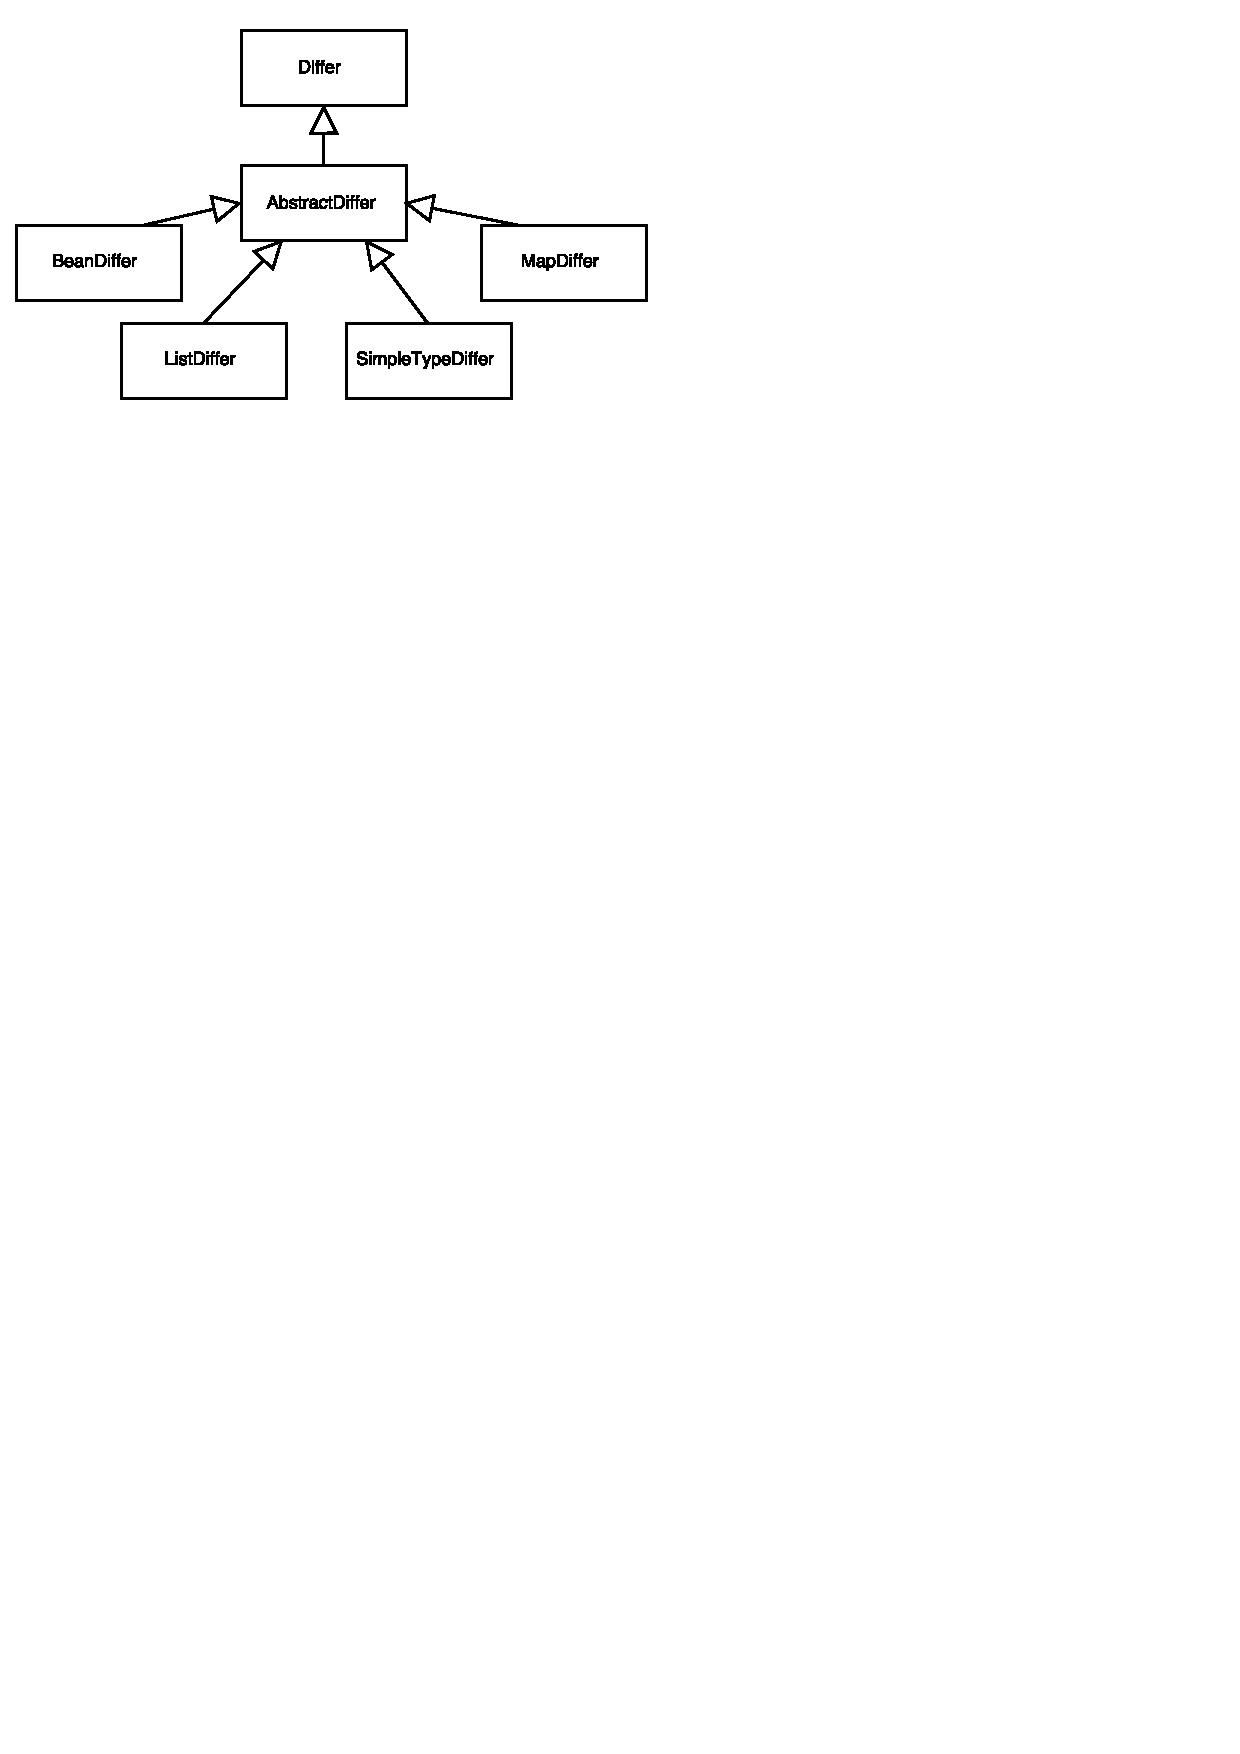
\includegraphics{differ-diagram.pdf}
        \end{center}
    \end{figure}
\end{frame}

\begin{frame}{Иерархия Декораторов}
    \begin{figure}
        \begin{center}
            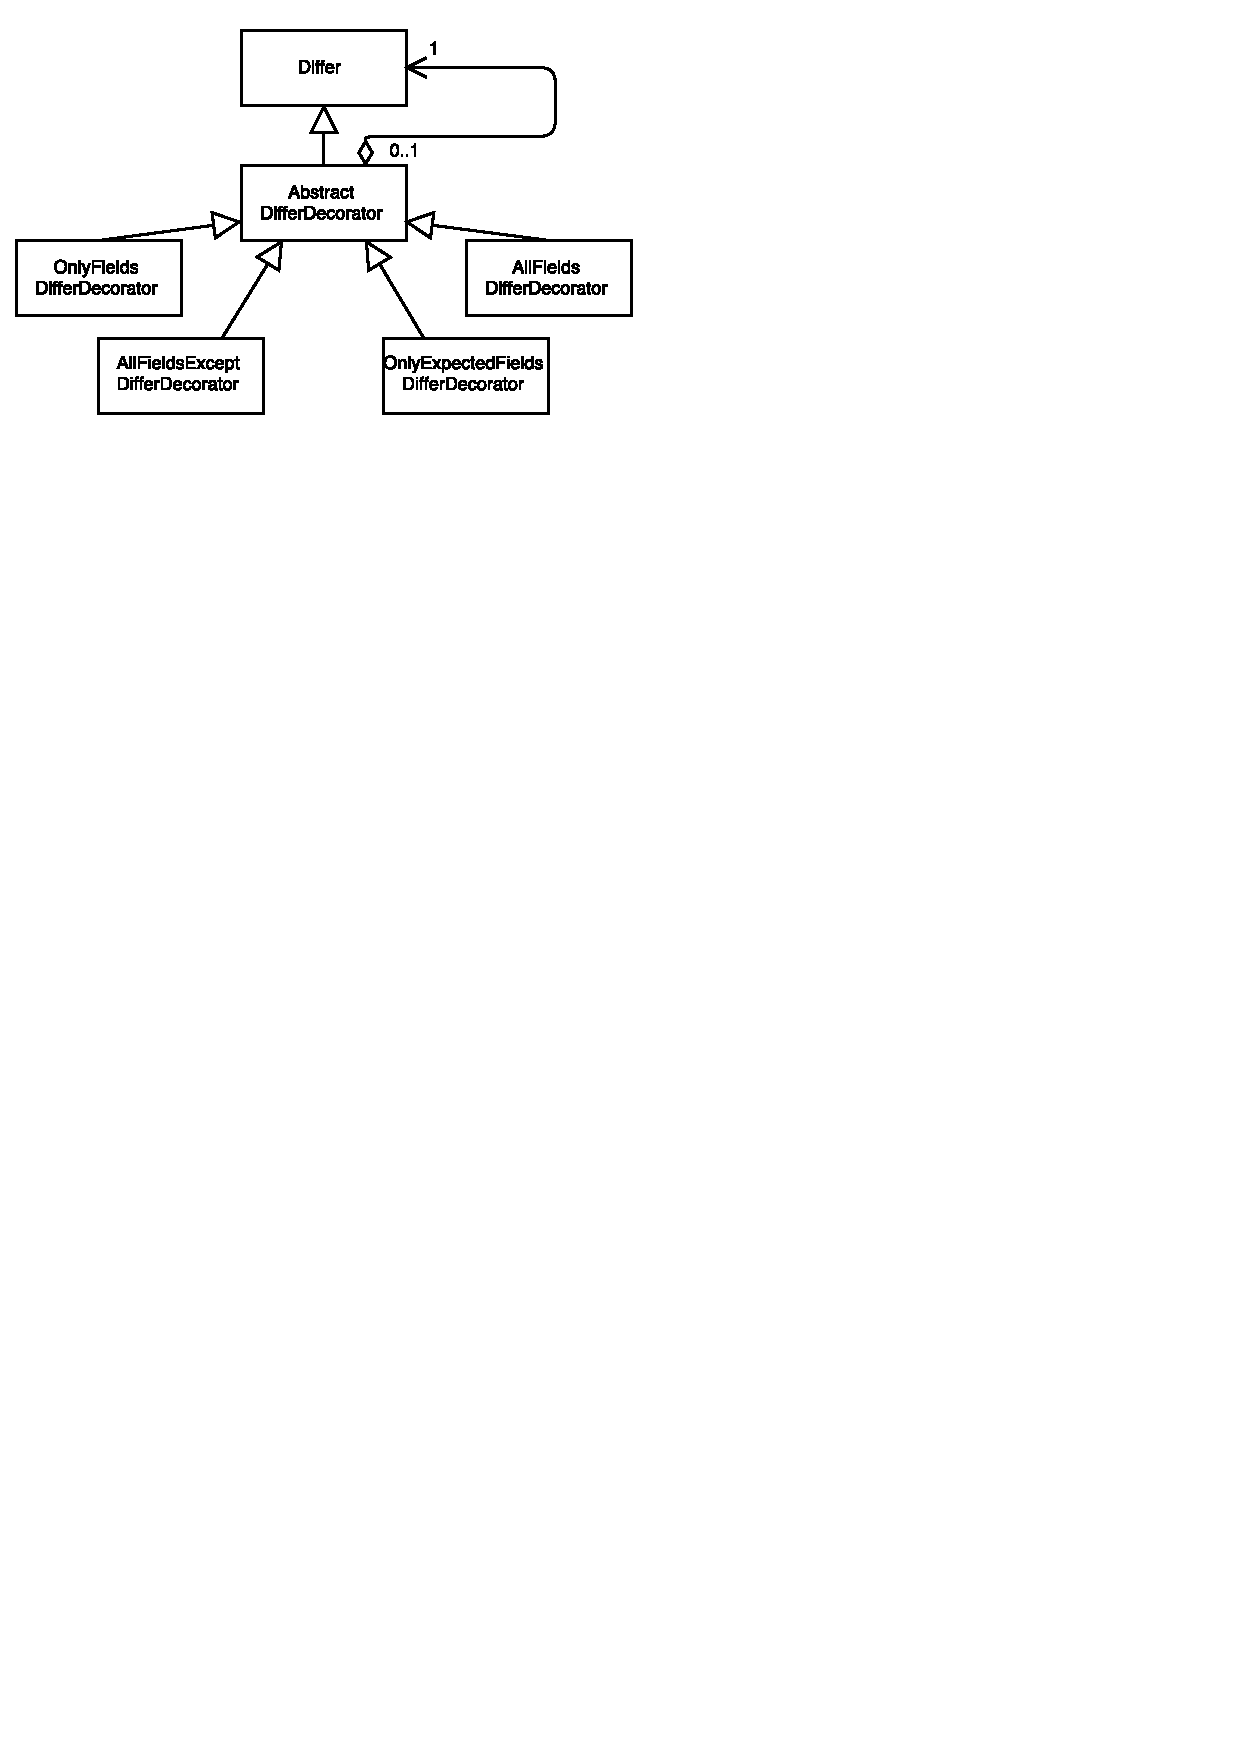
\includegraphics{decorator-diagram.pdf}
        \end{center}
    \end{figure}
\end{frame}

\begin{frame}{Классы стратегий}
    \begin{figure}
        \pause
        \begin{itemize}
            \item {DefaultCompareStrategy~--- стандартная стратегия \pause}
            \item {AllFieldsDefaultCompareStrategy \pause}
            \item {AllFieldsExceptDefaultStrategy \pause}
            \item {OnlyFieldsDefaultCompareStrategy \pause}
            \item {OnlyExpectedFieldsDefaultCompareStrategy}
        \end{itemize}
    \end{figure}
\end{frame}

\begin{frame}{Другие классы}
    \begin{figure}
        \pause
        \begin{itemize}
            \item {BeanFieldPath~--- путь поля \pause}
            \item {BeanField~--- поле \pause}
            \item {Diff~--- разница между полями}
        \end{itemize}
    \end{figure}
\end{frame}

\subsection{Дополнение текущей реализации}

\begin{frame}{Как реализовать Differ?}
    \pause
    \begin{itemize}
        \item {Следует реализовать метод compare \pause}
        \item {Ситуации, когда параметры равны null или <<значение отсутствует>>, обрабатывать не нужно \pause}
        \item {Следует пройтись по всем полям и использовать для них Differ в соответствии со стратегией}
    \end{itemize}
\end{frame}

\begin{frame}{Как реализовать декоратор для Differ?}
    \pause
    \begin{itemize}
        \item {Предполагается, что существующих декораторов хватает \pause}
        \item {Декоратор обязан корректно обрабатывать ситуации, когда одно из значений compare равно null \pause}
        \item {Декоратор обязан корректно обрабатывать ситуации, когда одно из значений <<отсутствует>>}
    \end{itemize}
\end{frame}

\begin{frame}{Как реализовать стратегию?}
    \pause
    \begin{itemize}
        \item {Следует реализовать метод getDefaultDiffer \pause}
        \item {Опционально: переопределить getCustomDiffer \pause}
        \item {Стратегия \textbf{обязана} возвращать Differ обёрнутый в декоратор \pause}
        \item {\textbf{Нельзя} переопределять getCustomOrDefaultDiffer}
    \end{itemize}
\end{frame}

\section{Результаты}

\subsection{Демонстрация BeanDiffer2}

\subsection{Заключение}

\end{document}
